\chapter{Geometry Part III}

\subsection{Worksheet 1C: Warm-Up Problems}

\textbf{Strategies Practice:} The SATs will test the same concept(s) in many different ways. Identify what area(s) the questions use. If you need help, then you can refer to the “About the math section at the beginning of this guide. Then, solve the questions.

\begin{multienumerate}
\mitemxx{\medium

Lauren and Rebecca leave Dave's house at the same time. Lauren walks east for an average at 6 miles per hour and continues for 3 hours. Rebecca scooters south for an average at 8 miles per hour for 3 hours. At the end of these 3 hours, what is the straight-line distance between them, in miles?

\begin{enumerate}[label=(\Alph*)]
\item 10
\item 18
\item 24
\item 30
\item 36
\end{enumerate}
}{\advanced

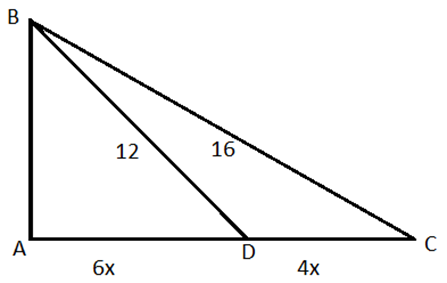
\includegraphics{34}

$\angle DAB$ is $90^\circ$. What is the length of $BA$?}
\end{multienumerate}

\vfill
\pagebreak
\section{Geometric Probability}

\begin{multienumerate}
\mitemxx{\basic

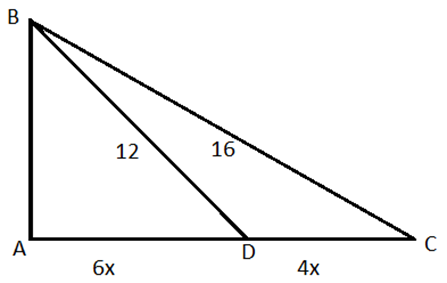
\includegraphics{34}

Note: Figure is not drawn to scale

\bigskip
In the figure above,$ B, D, F$, and $H$ are midpoints of $AC, CE, EG$, and $GA$, respectively. If a marble is thrown randomly and lands in rectangle $ACEG$, what is the probability that it lands on the shaded region?

\begin{enumerate}[label=(\Alph*)]
\item 1/4
\item 2/3
\item 1/2
\item 3/4
\item 4/5
\end{enumerate}
}{\medium

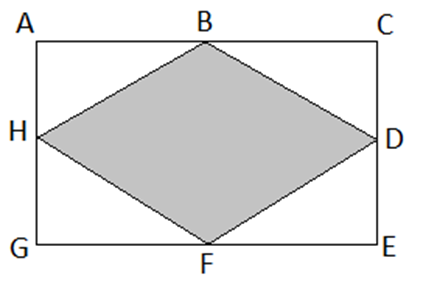
\includegraphics{35}

Three circles with the same center but different radii are combined to make the circular dartboard in the figure above. The circle enclosing the 1 point region has a radius that is two times bigger than the 3 point region and three times bigger than the 5 point region. If a dart thrown at random lands on the board, what is the probability that the person will get 3 points?

\begin{enumerate}[label=(\Alph*)]
\item 1/4
\item 2/11
\item 1/5
\item 1/3
\item 3/13
\end{enumerate}}
\end{multienumerate}

\hrulefill

\bigskip
Geometric probability uses probability concepts (the chance of an event occurring) to analyze shapes (which you use to find the chance of all possible events occurring).

\bigskip
The general formula is:

\vfill
\pagebreak
\subsection{SAT Worksheet 2C: 6 Questions, 8 Minutes}

\begin{multienumerate}
\mitemxx{\basic
\centerline{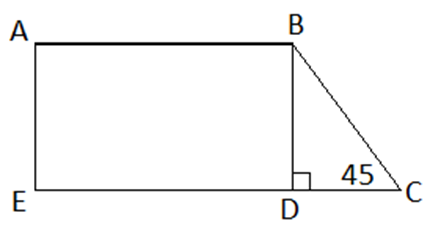
\includegraphics{37}}

In the figure $ABCDE$ above, $(1/2)AB=BD=5$ and $\angle C=45^\circ$. If a marble is rolled randomly and lands on the figure $ABCDE$, what is the probability that it lands on triangle $BCD$?

\begin{enumerate}[label=(\Alph*)]
\item 1/12
\item 1/10
\item 1/6
\item 1/5
\item 1/4
\end{enumerate}}{\basic

\centerline{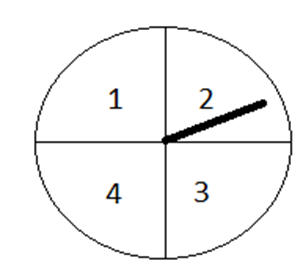
\includegraphics{38}}

If the circular spinner above was changed to have 6 identical sectors instead of 4, what is the probability of spinning twice and each time getting a number greater than 3?

\begin{enumerate}[label=(\Alph*)]
\item 1/4
\item 1/3
\item 1/6
\item 1/2
\item 2/3
\end{enumerate}}

\vfill
\mitemxx{\medium

\centerline{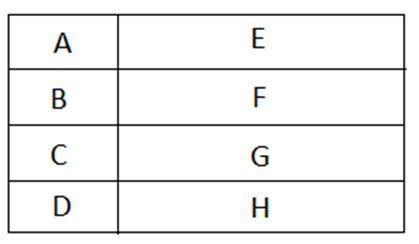
\includegraphics{39}}

In the figure above, boxes $A, B, C$, and $D$ are congruent. Box $E$ is 4 times bigger than box $A$ and is congruent to boxes $F, G$, and $H$. Two darts are thrown at the figure at random and lands on two of the boxes. What is the probability that Box E is hit both times?
}{\medium

\centerline{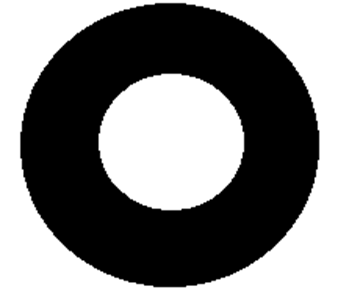
\includegraphics{40}}

\centerline{Note: Figure is not drawn to scale}

\bigskip
If the black ring has a diameter of 6 and the white ring inside the larger circle has a diameter of 4, what is the ratio of area of the black ring to the white ring?

\begin{enumerate}[label=(\Alph*)]
\item $9:4$
\item $3:2$
\item $5:1$
\item $11:3$
\item $6:1$
\end{enumerate}}

\vfill
\mitemxx{\advanced

\centerline{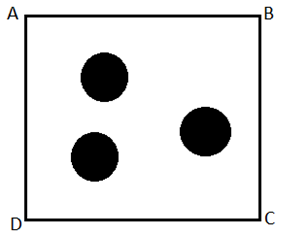
\includegraphics{41}}

The figure above shows the top view of an open square box that has an edge of length $l$. Each of the 3 circles have a diameter of length $l/2$. When a marble is into the box at random, it falls on either the circles or the background. What is the probability that the marble will not fall in one of the circles?

\begin{enumerate}[label=(\Alph*)]
\item $1-(3\pi/16)l$
\item $1-(1/4)l$
\item $(1/4)\pi l$
\item $1-\pi/16$
\item $1-(3/4)\pi l$
\end{enumerate}}{\advanced

An artist paints one side of a rectangular piece of cardboard 3 different colors, red, green, and blue. First, he paints 1/5 of the cardboard red. Then, he paints the remaining piece of cardboard equal parts red, green, and blue (none of the colors overlap). If a marble is rolled randomly on the cardboard, what is the probability that it will land on a space that is red rounded to the nearest hundredth?}
\end{multienumerate}

\vfill
\pagebreak
\section{Geometry Mixed Review}

\textbf{Strategy Recap}

\begin{itemize}
\item Strategy \#1: Draw a diagram. If one is already provided, then label the diagram.

\bigskip
\hrulefill

When a line represented by the expression $y+2x+5=0$ is plotted on a $xy$-coordinate graph, the line passes through which quadrants on the $xy$-coordinate graph?

\begin{enumerate}[label=(\Alph*)]
\item I only
\item I and III only
\item II only
\item I, II, and III only
\item I, II, III, and IV
\end{enumerate}

\hrulefill

\bigskip
\item Strategy \#2: Recognize what topic(s) the question is testing. Remember that the more difficult problems on the test will often combine two medium level topics.

\bigskip
\hrulefill

\begin{multicols}{2}
a) In the figure on the left, lines $l$ and $k$ are parallel. If $a=-3$, what is the value of $b^\circ$?

\vfill
b) What math content areas are used to solve this problem?

\vfill

\columnbreak
\centerline{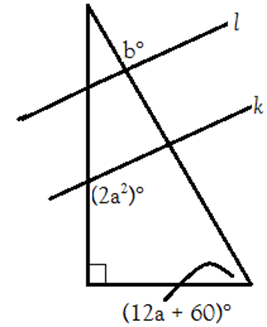
\includegraphics{42}}
\end{multicols}
\hrulefill

\bigskip
\item Strategy \#3: After you solve for your answer, make sure that what you selected matches what the question is asking for. This is critical in problems that require solving for variables.

\bigskip
\hrulefill

The diagonal of rectangle $ABCD$ is $2\sqrt{5}$ and the length of the rectangle is twice its width. What is the area of the rectangle?

\vfill
\hrulefill
\end{itemize}

\pagebreak
\subsection{SAT Worksheet 3C (Basic): 6 Questions, 8 Minutes}

\begin{multienumerate}
\mitemxx{If the area of a circle is 6 square inches, what is the perimeter of the circle?

\begin{enumerate}[label=(\Alph*)]
\item $12\pi$
\item $4\pi$
\item $2\sqrt{6}\pi$
\item $6\pi$
\item $\sqrt{6}\pi$
\end{enumerate}}{If the sum of the circumferences of two congruent circles is $40\pi$, what is the radius of one of the circles?

\begin{enumerate}[label=(\Alph*)]
\item 4
\item $4\pi$
\item 8
\item 10
\item 20
\end{enumerate}}

\vfill
\mitemxx{A town is building a water tower and wants to build a tower that can hold the most water. Which of the following designs would hold the most water?

\begin{enumerate}[label=(\Alph*)]
\item Rectangular prism with length and height of 3 and width of 6
\item Cube with length 5
\item Rectangular prism with a base area of 4.5 and height of 10
\item Cylinder with a radius of 2 and height of 4
\item Triangular prism with a base of 4, altitude of 5, and height of 10
\end{enumerate}}{Points $A, B$, and $C$ lie on a circle whose center is $D$ and radius of 5. If the measure of $\angle ADB$ is $45^\circ$, what is the length of arc $AB$?

\begin{enumerate}[label=(\Alph*)]
\item $\pi/2$
\item $1.25\pi$
\item $1.50\pi$
\item $1.75\pi$
\item $2.0\pi$
\end{enumerate}}

\vfill
\mitemxx{

\medskip
\centerline{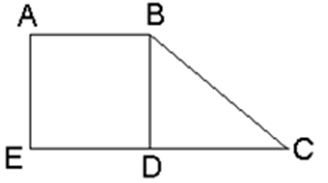
\includegraphics{43}}

One side of square $ABDE$ is 2. Angle C is $45^\circ$. What is integer closest to the perimeter of shape $ABCDE$?}{

\medskip
\centerline{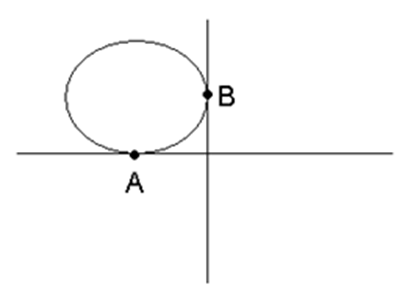
\includegraphics{44}}

The above figure is a circle that is tangent to points $A$ and $B$. If $B$ has coordinates $(0, 3)$, then what is the $x$-coordinate of Point $A$?}
\end{multienumerate}

\vfill
\pagebreak
\subsection{SAT Worksheet 4C (Medium): 6 Questions, 9 Minutes}

\begin{multienumerate}
\mitemxx{Points $A$ and $B$ lie on a circle whose center is $D$. If the area of the sector enclosing $AB$ is $9\pi$ square meters and the area of the full circle is $36\pi$ square meters, what is the measure of the arc length $AB$?

\begin{enumerate}[label=(\Alph*)]
\item $\pi$
\item $2\pi$
\item $3\pi$
\item $5\pi$
\item $9\pi$
\end{enumerate}}{A cube has an edge of $2x$. What is the total surface area of the cube?

\begin{enumerate}[label=(\Alph*)]
\item $24x^2$
\item $12x^2$
\item $10x^2$
\item $8x^2$
\item $8x^3$
\end{enumerate}}

\vfill
\mitemxx{Marlene currently starts at her house and drives 5 miles west, then 12 miles north and then 6 miles west to get to her work. How much longer is this route, in miles, than the number of miles in the route directly from her house to her work, rounded to the nearest hundredth?}
{A vase in the shape of a rectangular prism has height 12 centimeters and a base with an area of 25 square centimeters. When the vase is 3/4 filled with water, what is the volume of the water?}

\vfill
\mitemxx{

\medskip
\centerline{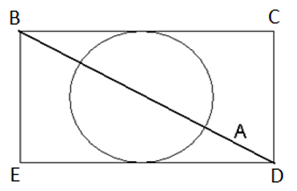
\includegraphics{45}}

A circle is inscribed inside of rectangle $BCDE$ in the figure $BC=8$ and the length of the diagonal, $A$, is 10. What is the radius of the circle?
\begin{enumerate}[label=(\Alph*)]
\item 3
\item 4
\item 8
\item 10
\item Unable to determine based on available information
\end{enumerate}}{The diameter of a circle is 5 inches more than its radius. What is the area of the circle, in square inches?


\begin{enumerate}[label=(\Alph*)]
\item 2.5
\item 5
\item 10
\item $12.25\pi$
\item $25\pi$
\end{enumerate}}
\end{multienumerate}

\pagebreak
\subsection{SAT Worksheet 5C (Advanced): 6 Questions, 10 Minutes}

\begin{multienumerate}
\mitemxx{A rectangular prism has a length of s square inches, a width of $2s$ square inches, and a height of $s$ square inches. What is the minimum number of square feet of wrapping paper in terms of $s$ would it take to wrap the entire shape?

\begin{enumerate}[label=(\Alph*)]
\item $6s^2$
\item $2s^3$
\item $6s^3$
\item $10s^3$
\item $12s^3$
\end{enumerate}}{If the diameter of a circle is doubled, by what percent will the area of the circle increase?

\begin{enumerate}[label=(\Alph*)]
\item $150\%$
\item $200\%$
\item $225\%$
\item $300\%$
\item $400\%$
\end{enumerate}}

\vfill
\mitemxx{A prism has the base of an equilateral triangle with a side length of 6. The height of the triangular prism is 8. What is the volume of the triangular prism?

\begin{enumerate}[label=(\Alph*)]
\item 9
\item 42
\item $72\sqrt{3}$
\item 144
\item $144\sqrt{3}$
\end{enumerate}}{Two cylindrical cans are stacked on top of each other. The height of a right circular cylinder is 6 and the diameter of the base is 10. Which of the following is a possible distance from the center of the base at the bottom to a point on the edge of the other can?

\begin{enumerate}[label=(\Alph*)]
\item 5
\item $\sqrt{61}$ (approximately 7.81)
\item 10
\item 12
\item 1
\end{enumerate}}

\vfill
\mitemxx{

\medskip
\centerline{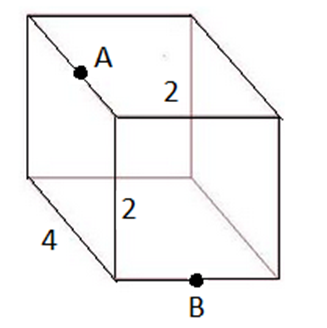
\includegraphics{46}}

The rectangular prism show above has a length and a height of 2, and a width of 4. If points $A$ and $B$ are midpoints of two edges, what is the length of $AB$?

\begin{enumerate}[label=(\Alph*)]
\item 2
\item $2\sqrt{2}$
\item $\sqrt{8}$
\item 3
\item Unable to determine based on available information
\end{enumerate}}{

\medskip
\centerline{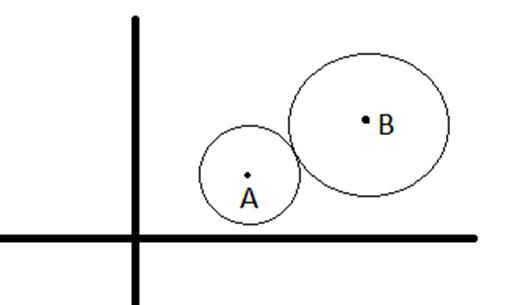
\includegraphics{47}}

In the figure above, there are two circles with centers $A$ and $B$ respectively. Line segment $AB=12$ and center $A$ has the coordinates $(4, 3)$. If the coordinates of center $B$ is $(7, b)$, what is the value of $b$, rounded to the nearest hundredth?}
\end{multienumerate}